\documentclass[12pt,spanish]{article}
\usepackage[spanish]{babel}
\selectlanguage{spanish}
\usepackage[utf8]{inputenc}
\usepackage{graphicx}
\title{Entrega 1}
\author{
  Lluch, Pablo\\
  \texttt{pablo.lluch@gmail.com}
  \and
  Fuentes, Tomás\\
  \texttt{tafuentesc@gmail.com}
  \and
  Teles, Nuno\\
  \texttt{nuno\_teles3@hotmail.com}
}

\begin{document}

\maketitle
\newpage

\section{Introducci\'on}
A continuación se presenta el informe de avance, que tiene como principal objetivo identificar, evaluar y analizar algoritmos avanzados que están directamente relacionados con el problema de encontrar k frequent itemsets, en grandes bases de datos. Para lograr este objetivo, se seleccionar\'an un conjunto de papers científicos. Estos papers constituyen parte de la investigación que se desarrolla actualmente en esta área y cada uno de ellos aborda una distinta estrategia. Esta estrategia intenta mejorar sucesivos problemas identificados en algoritmos anteriores y/o hacer mejorías que hagan que su implementaci\'on sea lo más simple posible, permitiendo al mismo tiempo encontrar una solución para el problema en el menor tiempo de ejecución.
\\\\
Por ejemplo, una medida de comparación comúnmente utilizada, consiste en comparar diferentes soluciones sobre distintas bases de datos: \emph{sparse} (baja fracci\'on de items presentes en cada transacci\'on) y densas (alta fracción de ítems presentes en cada transacción).Desde ahí se extrapolan conclusiones sobre los datos. En general, cuando se aborda este tipo de problema, estamos interesados en descubrir cu\'ales son los algoritmos que presentan menores tiempos de ejecución. Sin embargo, el análisis de revisión bibliogr\'afica que se hizo en el presente informe muestra que no necesariamente el algoritmo que en un comienzo presenta mejor tiempo de computación en distinta bases de datos es el mejor y más simple de implementar. A veces, hay algoritmos que son muy rápidos pero emplean una estructura de datos muy compleja lo que torna difícil su implementación y además requieren cargar completamente la base de datos de transacciones en memoria. Es posible observar que ciertas alternativas cuando se aplican en determinados conjuntos de datos pueden mantener su eficiencia y generar  más ventajas en t\'erminos de implementación. Son esas alternativas, ventajas y desventajas que intentaremos discutir  y evaluar en este informe consider\'andolas al momento de seleccionar nuestro modelo para el proyecto.
\\\\
Este informe se presentará en diferentes secciones, primero, con la identificación del problema (asociado al concepto de itemsets frecuentes) y posteriormente para cada unos de los algoritmos revisados, se har\'a una descripción general del método y se identificar\'a cual es su objetivo así como ventajas y desventajas comparativas. Finalmente,  se describirá con mayor detalle el modelo que utilizaremos en el proyecto de Minería de Datos.
En las siguientes secciones y en la bibliograf\'ia se podr\'an encontrar los papers investigados.

\section{Problema}

El problema de encontrar k itemsets frecuentes en grandes volúmenes de información ha sido un importante foco de investigación a lo largo de los últimos años, durante los cuales se han propuesto distintas implementaciones y algoritmos que buscan solucionar este problema, algunos de los cuales son puramente optimizaciones de otros algoritmos más tradicionales.
\\\\
Esta técnica para minar datos es un método de análisis bastante conocido que busca encontrar correlaciones y tendencias en los datos para después ayudar a las empresas en la toma de decisiones  y optimización de sus procesos.
\\\\
Dada una base de datos con N transacciones, cada una con un conjunto de ítems, el proceso de encontrar los k- itemsets frecuentes en una base de datos se resume a identificar todos los itemsets en que el soporte de éste sea mayor a un umbral mínimo dado por el usuario. 

\section{SAM}
\subsection{Objetivo}
El objetivo del Algoritmo SAM (Split and Merge)  es encontrar todos los posibles itemsets frecuentes dada una base de datos y un umbral positivo. Al contrario de algunos algoritmos basados en A-priori, este algoritmo usa un modelo distinto para procesar los datos consistente una busca en profundidad a través una estrategia comúnmente observada en algoritmos computacionales - dividir para conquistar. Así, para un determinado ítem a considerar, cada sub-problema consiste en encontrar todos los itemsets que contienen al ítem usando para eso un conjunto de transacciones  más pequeño también designado de base de datos condicional (conjunto de transacciones que contiene el item).Todos los itemsets que no contienen el ítem a considerar constituyen también un sub-problema válido y por lo tanto, una base de datos condicional en la cual buscamos una solución. La gracia del algoritmo es usar esta idea e iterar recursivamente sobre cada un de estos sub-problemas y encontrar todos los itemset frecuentes.

\subsection{Descripci\'on}
El SAM es un de los algoritmos que pertenece a la categoría de los algoritmos de eliminación recursiva que son utilizados para obtener conjuntos de itemsets frecuentes. Muy idéntico al algoritmo RELIM,  ambos se basan en el mismo principio al momento procesar los itemsets. A diferencia de RELIM que usa una representación parcial vertical de los datos, SAM usa un único arreglo que mantiene en cada posición todas las listas de ítems (transacciones). Este arreglo es procesado al inicio del algoritmo usando dos operaciones Split and Merge, operaciones que tratan de construir sucesivamente las base de datos condicionales que son usadas en la recursión.

Para construir el arreglo que va servir de input al algoritmo es necesario pre-procesar las transacciones inicialmente y por eso, se procede a un conjunto de pasos. En primer lugar se determinan las frecuencias de cada uno de los ítems individualmente, de forma eliminar los ítems que son infrecuentes. Después de este paso, se ordenan cada un de los ítem presentes en cada transacción de forma creciente para poder minimizar su tiempo de ejecución. Por fin, se  modifica el orden de presentación de las transacciones en la base de datos siguiendo un orden lexicográfico descendente. La estructura de datos que guarda esta información se construye a través de un arreglo que tiene para cada posición cada transacción, respectando el orden obtenido anteriormente y un contador que representa el numero de ocurrencias de esa misma transacción.

Con la ayuda de la operación de Split, en cada paso de la recursión conseguimos expandir el prefijo de cada base de datos condicional. A esto se debe que esta operación permite una separación del ítem líder de sus restantes elementos construyendo un sub-problema de menor dimensión que consiste en las transacciones que contienen el ítem líder pero en el que este ítem fue removido. Este sub-problema es procesado independientemente sobre un nuevo arreglo de forma recursiva. Así se consigue encontrar todos los itemset frecuentes que contienen el ítem líder bastando para eso, preguntar en cada paso se el ítem de separación es frecuente. Su suporte es computado sumando todos los suportes de las transacciones que lo contienen. 
Por otro lado, se usa el arreglo obtenido en el paso anterior (de separación)  para construir un nuevo arreglo que representa las transacciones que no contienen el ítem. Este nuevo arreglo  resulta de la Operación Merge responsable por combinar el arreglo obtenido con la Operación Split y el resto del arreglo original que como sabemos no fue separado y por lo tanto es necesario para descubrir todos los ítem sets frecuentes que no contienen el ítem líder. Esta operación tiene como principal objetivo combinar posibles transacciones que tengan el mismo ítem líder y agrupar transacciones iguales reduciendo el numero de objetos a procesar. Este arreglo es después procesado recursivamente.

\subsection{Ventajas}

- Su estructura de datos es bastante simples porque engloba apenas un arreglo para almacenar la información a procesar y por eso, hace que el algoritmo pueda ser utilizado con almacenamiento  externo (por ejemplo tabla) evitando casos que el algoritmo no pueda funcionar porque no existe espacio para cargarlo en memoria principal.

- Además, durante las Operaciones de Split y Merge en cada paso de recursión, apenas es necesario copiar el contador de ocurrencias de transacciones y el puntero incrementado para un nuevo arreglo lo que hace que en final sea necesario una única copia de las transacciones. Por fin, hay que notar el bajo consumo memoria visto que en cada paso de la recursión sólo es necesario alocar un único arreglo que resulta de la Operación Split  del  arreglo pasado como input ya que este arreglo puede ser utilizado para separar el próximo ítem cuando el algoritmo fuer ejecutado nuevamente en la recursión.

\subsection{Desventajas}

- Puede acontecer que la operación de merge atrase el algoritmo cuando las listas de transacciones presenten tamaños diferentes.

\section{BitTable}

\subsection{Objetivo}

El objetivo de este algoritmo consiste en optimizar el uso de memoria y tiempo en el que caen los algoritmos basados en A-Priori. Para lo anterior, los autores proponen una nueva estructura de datos conocida como BitTableFI, la cual permite representar la base de datos como una representación vertical comprimida de la BD, en la que cada registro asociado a un determinado ítem es un arreglo de bits en el que una entrada es 1 si el ítem está en dicha tupla ó 0 en caso contrario.
\\\\
Gracias al uso de esta estructura se logró un considerable ahorro en memoria a la vez que se mejoró el tiempo de ejecución del algoritmo, mayormente gracias a la velocidad propia de las operaciones bitwise en comparación con sus equivalentes en la representación original.

\subsection{Descripción}

En el año 2007, Dong \& Han propusieron un nuevo algoritmo para extraer itemsets frecuentes llamado BitTableFI. Más allá del algoritmo utilizado, el gran aporte de su trabajo son las estructuras de datos que utilizan para comprimir la base de datos y los itemsets frecuentes en cadenas de bits. El algoritmo se puede separar en 4 grandes pasos: primero, se identifican los items frecuentes, descartando los que no cumplan con el soporte mínimo ($L_1$). Posterior a esto se comprime la base de datos considerando sólo estos items frecuentes, obteniendo una representación vertical comprimida de ésta conocida como BitTable. En tercer lugar, se obtienen los itemsets frecuentes en el cual cada set está compuesto por 2 items frecuentes ($L_2$). Finalmente, el cuarto paso es un proceso iterativo el cual se puede subdividir en 2 sub etapas: generación de candidatos y cálculo de soporte. Este último paso se repite hasta que no se puedan obtener más candidatos.
\\\\
Para comprimir la base de datos y transformarla en la BitTable, ésta se debe comprimir tanto de forma vertical como horizontal. Para realizar lo anterior, primero codificamos cada tupla de la tabla como un arreglo de bits, donde el valor de la i-ésima posición es 1 si la tupla contiene al ítem i ó 0 en caso contrario. Una vez hecho esto, construimos la BitTable de la BD la cual poseé una entrada por cada ítem frequente donde el valor de la i-ésima entrada está dado por el arreglo de bits formado al considerar los bits de todas las tuplas en la columna del i-ésimo ítem frequente.
\\\\
Una vez obtenida la BitTable, obtenemos el itemset frecuente en el que cada itemset posee exactamente 2 items frecuentes ($L_2$). Posterior a esto, cada itemset es representado como un arreglo de bits de largo igual a la cantidad de items frecuentes en $L_1$, donde el i-ésimo bit es 1 si el i-ésimo ítem es parte de éste.
\\\\
Una vez obtenidas la BitTable y $L_2$ procedemos a calcular $L_k$, en el cual cada itemset está compuesto por k items. El cálculo de $L_k$ se realiza de la siguiente forma: para cada itemset en $L_{k-1}$, se toma el primero y se cambia el último 1 de su representación por un 0 (A esta representación intermedia se le llama MID). Posterior a esto, se hace un and bitwise (\&) entre el MID y el siguiente itemset después de éste. Si el valor retornado es MID, entonces ambas representaciones tienen un item de diferencia, por lo que las mezclamos y lo agregamos a $L_k$; en caso contrario, se descarta. Este proceso se repite para todos los itemsets que están después del itemset con el cual se contruyó el MID. Una vez comparados con todos, se toma el itemset que viene después del MID, se saca el MID de éste y se repite el proceso hasta haber probado con todos los itemsets de $L_{k-1}$.
\\\\
Una vez obtenido $L_k$ se calcula su soporte para cada itemset dentro de éste realizando un and bitwise (\&) entre las columnas de la BitTable asociadas a los ítems dentro de ésta y contando la cantidad de 1's en el resultado. Hecho esto, se eliminan los itemsets que no superen el soporte mínimo establecido. Si la cantidad de itemsets en $L_k$ al final de la poda es mayor a cero, se continúa con $L_{k+1}$; en caso contrario, el algoritmo se detiene ahí. En la Figura 1 se puede ver el pseudo código del algoritmo.

\begin{figure}
\centering
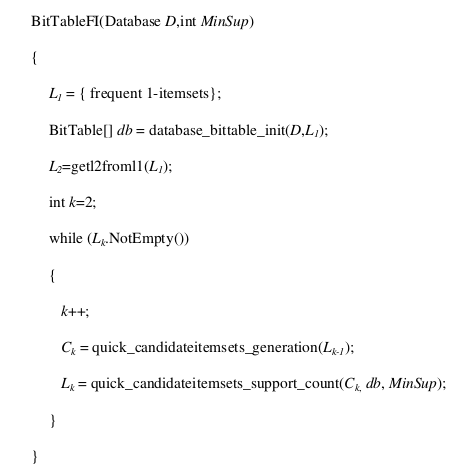
\includegraphics[scale=0.8]{bittablefi.png}
\caption{BitTable pseudo-algorithm}
\end{figure}

\subsection{Ventajas}

\begin{enumerate}
\item Ahorro en memoria: Gracias a la compactación de la base de datos en la forma de la BitTable se disminuye considerablemente el tamaño de la base de datos en disco (se habla  de disminuciones del orden de 1/160 \cite{bit_table}).
\item Ahorro en tiempo: Gracias al menor tamaño de la BD se pueden cargar segmentos más grandes en memoria, lo cual disminuye los accesos a disco. Adicionalmente, el uso de operaciones bitwise para determinar los itemsets candidatos y calcular el soporte de éstos resulta mucho más eficiente que las típicas operaciones de conteo realizadas sobre la representación original, lo cual significa un sustancial boost en el rendimiento del algoritmo. 
\end{enumerate}

\subsection{Desventajas}

\begin{enumerate}
\item El algoritmo propuesto es, en realidad, el mismo algoritmo A-priori. La única diferencia real es la estructura de datos utilizada, la cual es responsable de la mejora en rendimiento obtenida. Así, es fácil deducir que este algoritmo no puede rendir mejor que aquellos de la línea de FP-Growth, los cuales son más rápidos puesto que solo traversan la base de datos 2 veces.
\item El uso de la BitTable puede ser difícil con otros algoritmos que ya tengan una estructura de datos propia tales como FIUT [*] y FP-Growth.
\end{enumerate}

\section{GarNet}

\subsection{Objetivo}

Abordar mediante m\'etodos de inteligencia artificial el problema de encontrar asosiaciones cuantitativas, que tratan con atributos continuos. La idea es evitar discretizaciones que generen p\'erdida de informaci\'on y sean complejas de calibrar.

\subsection{Descripción}

El objetivo de GarNet \cite{gene} consiste en lograr encontrar asosiaciones entre genes para armar una red de genes, la cual consiste en un grafo cuyos nodos son determinados genes y sus vínculos corresponden a asociaciones entre ellos.
\\ \\
Para trabajar con información acerca de los genes, se utiliza comúnmente tecnología basada en \emph{microarrays}, los cuales permiten obtener genotipos, medir niveles de expresión de genes y otros fines relacionados. Particularmente, interesa saber qué genes están interactuan con otros, en el sentido de que un gen puede codificar una proteína o ARN que interactúa con el producto de otro. Para esto se puede formar una red de regulación génica, que es un grafo que establece estas relaciones.
\\\\
Este es un problema que puede ser potencialmente atacado usando reglas de asociación. Sin embargo, una de las dificultas es que la información que se obtiene de los \emph{microarrays} son atributos continuos que contienen informaci\'on de la concentraci\'on de nucle\'otidos expresados en moles. Para atacar este tipo de problemas, una opci\'on es discretizar el valor de las variables. Sin embargo, escoger una buena discretizaci\'on puede ser complejo, sobre todo si adem\'as los rangos de valores para cada atributo son muy distintos. GarNet \cite{gene} pretende atacar este problema encontrando reglas de asociaaciones cuantitativas (o QAR), que trabajan con intervalores continuos. Las asociaciones, en este caso, vienen a ser del tipo ($A \in [a,b], B \in [c, d] => C \in [e, f]$)
\\\\
De modo general, GarNet es un algoritmo para encontrar asociaciones entre genes basado en el algoritmo genético NSGA II \cite{nsga}. NSGA II es un algoritmo genético eficiente que permite trabajar con múltiples objetivos. En general, los algoritmos genéticos permiten encontrar soluciones a problemas que no tienen un planteamiento matemático simple, y que usa búsquedas estocásticas para analizar un espacio de búsqueda amplio, como es el caso de este problema. 
\\\\
Para este problema en particular, los autores de \cite{gene} crea una población de individuos que son equivalentes cada uno a una regla de asociación posible. Si tenemos un total de $n$ atributos, un cromosoma consistir\'a en dos partes de largo n cada una: La primera indica el intervalo con el que estamos trabajando para cada atributo, mientras que la segunda parte consiste en $n$ n\'umeros que pueden tomar los valores 0, 1 y 2. Si el valor es 0, implica que el atributo asociado no participa de la regla de asociaci\'on. Si el n\'umero es 1, entonces el (o los) atributos forman parte del antecedente de la regla de asociaci\'on. Finalmente, si el n\'umero es 2, entonces el atributo forma parte del consecuente de la regla. Como ejemplo, si tenemos el individuo de la Fig. 1, equivaldr\'ia a tener la regla de asociaci\'on $CLB1 \in [-0.68, 0.05], CLN2 \in [-1.11, 0.00] => CLB5 \in [-0.85, 0.10]$
\\

\begin{figure}
\centering
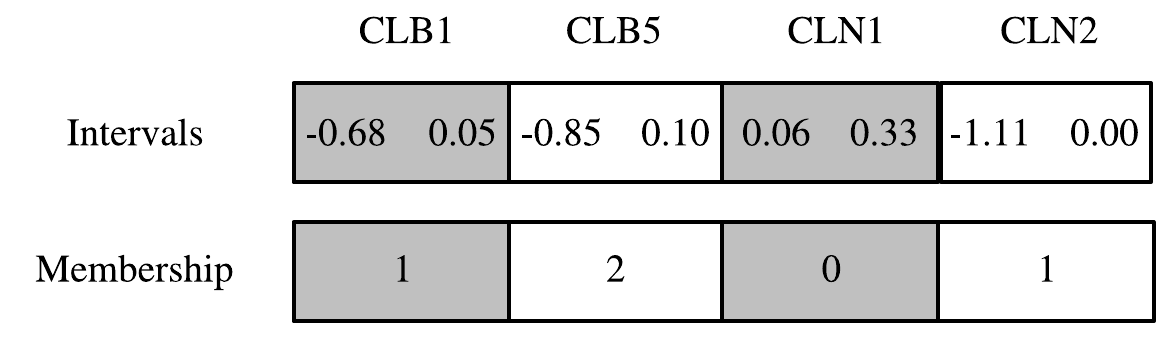
\includegraphics[scale=0.4]{association.png}
\caption{Cromosoma}
\end{figure}

Para dise\~{n}ar un algoritmo gen\'etico, se necesitan definir:

\begin{enumerate}
\item Operador de Crossover - permite generar mezclas entre los distintos individuos. Aqu\'i, por ejemplo, se puede intercambiar la posici\'on de una de las partes de una regla de asociaci\'on por la parte de otra.
\item Operador de mutaci\'on - permite mutar o cambiar aleatoriamente a un individuo para generar mayor diversidad. Los autores de \cite{gene}, por ejemplo, definieron un operador de mutaci\'on que permite cambiar el lado de la regla de asociaci\'on en que aparece un atributo dado, adem\'as de modificar el intervalo de los atributos.
\item Condici\'on de t\'ermino - Define la cantidad de iteraciones antes de terminar con el algoritmo. En este caso en particular, no se menciona la cantidad de iteraciones. Sin embargo, como cada proceso evolutivo produce un regla de asociaci\'on, los autores ejecutan el proceso completo varias veces hasta obtener un set de reglas de asociaciones candidatas.
\item Funci\'on de fitness - Nos sirve medir qu\'e tan bueno es un individuo, pues en un algoritmo gen\'etico se seleccionan ciertos individuos de una poblaci\'on con mayor o menor probabilidad de acuerdo a este criterio. En este paper, se utilizan medidas cl\'asicas asociadas a las reglas de asociaci\'on, vale decir, el soporte, confianza, y un valor de accuracy que describe qu\'e tanto se ajusta la regla encontrada a los datos reales que tenemos.
\end{enumerate}


Adicionalmente, el proceso se repite utilizando distintos datasets. Una vez se obtienen una cierta cantidad de reglas de asociaciones predefinidas, se intersectan los pares de atributos encontrados para cada dataset.

\subsection{Ventajas}
\begin{enumerate}
\item Los rangos de los atributos son variables y no es necesario definir previamente muchos par\'ametros ni tener en cuenta el rango de valores de los atributos
\item Permite resolver un problema complejo que un algoritmo como Apriori no podr\'ia encontrar midiendo solamente niveles de soporte y confianza
\item Uso de memoria no es elevado
\item Estructuras de datos usadas son relativamente simples
\item Permite buscar un espacio de hip\'otesis alto
\end{enumerate}

\subsection{Desventajas}
\begin{enumerate}
\item Complejidad computacional alta por la cantidad de iteraciones que se deben ejecutar normalmente en un algoritmo gen\'etico
\item Al ser un proceso de b\'usqueda estoc\'astico no se garantiza optimalidad
\item Puede ser complejo definir los operadores gen\'eticos adecuados
\item Aborda un problema no muy general
\end{enumerate}

\begin{thebibliography}{9}

	\bibitem{gene}
	M. Martínez-Ballesteros, I.A. Nepomuceno-Chamorro, J.C. Riquelme,
	Discovering gene association networks by multi-objective evolutionary quantitative association rules,
	Journal of Computer and System Sciences 80, 2014,
	pp. 118-136

	\bibitem{bit_table}
	BitTableFI: An efficient mining frequent itemsets algorithm
	Jie Dong, Min Han,
	School of Electronic and Information Engineering, Dallan University of Technology, Dalian 116023,

	\bibitem{dhp}
	An effective Hash-Based Algorithm for Mining Association Rules
	Jong Soo Park, Ming-Syaen Chen,
	IBM Thomas J. Watson Research Center

	\bibitem{nsga}
	Aravind Seshadri,
	A Fast Elitist Multiobjective Genetic Algorithm: NSGA-II

	\bibitem{relim}
	Christian Borgelt
	Keeping Things Simple: Finding Frequent Item Sets by Recursive Elimination

	\bibitem{sam}
	Christian Borgelt
	Simple Algorithms for Frequent Item Set Mining

\end{thebibliography}
\end{document}